\documentclass{standalone}
\usepackage{tikz}
\usetikzlibrary{patterns, positioning}

\begin{document}
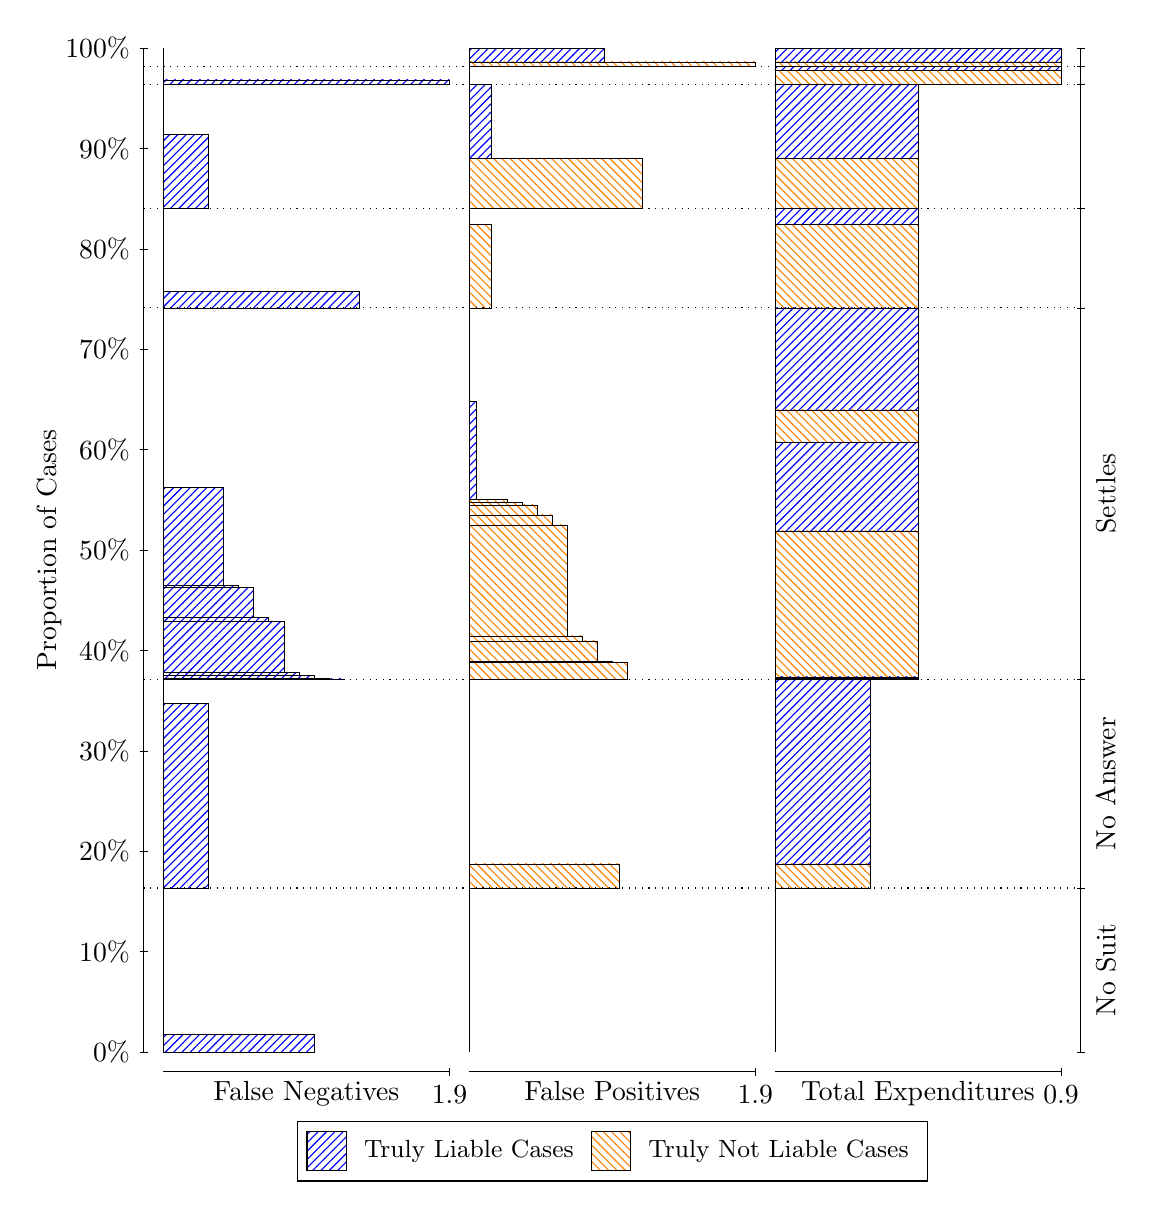
\begin{tikzpicture}
\draw[black, very thin] (1.5,1.75) -- (1.5,14.5);
\node[rotate=90, anchor=center] at (0.3, 8.125) {Proportion of Cases};
\draw[black, very thin] (1.45,1.75) -- (1.55,1.75);
\node[anchor=east] at (1.45, 1.75) {0\%};
\draw[black, very thin] (1.45,3.025) -- (1.55,3.025);
\node[anchor=east] at (1.45, 3.025) {10\%};
\draw[black, very thin] (1.45,4.3) -- (1.55,4.3);
\node[anchor=east] at (1.45, 4.3) {20\%};
\draw[black, very thin] (1.45,5.575) -- (1.55,5.575);
\node[anchor=east] at (1.45, 5.575) {30\%};
\draw[black, very thin] (1.45,6.85) -- (1.55,6.85);
\node[anchor=east] at (1.45, 6.85) {40\%};
\draw[black, very thin] (1.45,8.125) -- (1.55,8.125);
\node[anchor=east] at (1.45, 8.125) {50\%};
\draw[black, very thin] (1.45,9.4) -- (1.55,9.4);
\node[anchor=east] at (1.45, 9.4) {60\%};
\draw[black, very thin] (1.45,10.675) -- (1.55,10.675);
\node[anchor=east] at (1.45, 10.675) {70\%};
\draw[black, very thin] (1.45,11.95) -- (1.55,11.95);
\node[anchor=east] at (1.45, 11.95) {80\%};
\draw[black, very thin] (1.45,13.225) -- (1.55,13.225);
\node[anchor=east] at (1.45, 13.225) {90\%};
\draw[black, very thin] (1.45,14.5) -- (1.55,14.5);
\node[anchor=east] at (1.45, 14.5) {100\%};

\draw[black, very thin] (13.4,1.75) -- (13.4,14.5);
\draw[black, very thin] (13.35,1.75) -- (13.45,1.75);
\node[anchor=west] at (13.35, 1.75) {};
\draw[black, very thin] (13.35,3.8331) -- (13.45,3.8331);
\node[anchor=west] at (13.35, 3.8331) {};
\draw[black, very thin] (13.35,6.482) -- (13.45,6.482);
\node[anchor=west] at (13.35, 6.482) {};
\draw[black, very thin] (13.35,11.201) -- (13.45,11.201);
\node[anchor=west] at (13.35, 11.201) {};
\draw[black, very thin] (13.35,12.461) -- (13.45,12.461);
\node[anchor=west] at (13.35, 12.461) {};
\draw[black, very thin] (13.35,14.04) -- (13.45,14.04);
\node[anchor=west] at (13.35, 14.04) {};
\draw[black, very thin] (13.35,14.27) -- (13.45,14.27);
\node[anchor=west] at (13.35, 14.27) {};
\draw[black, very thin] (13.35,14.5) -- (13.45,14.5);
\node[anchor=west] at (13.35, 14.5) {};

\draw[black, very thin, pattern color=blue, pattern=north east lines] (1.75,1.75) rectangle (3.6623,1.9692);
\draw[black, very thin, pattern color=orange, pattern=north west lines] (1.75,1.9692) rectangle (1.75,3.8331);
\draw[black, very thin, pattern color=blue, pattern=north east lines] (1.75,3.8331) rectangle (2.3237,6.1768);
\draw[black, very thin, pattern color=orange, pattern=north west lines] (1.75,6.1768) rectangle (1.75,6.482);
\draw[black, very thin, pattern color=blue, pattern=north east lines] (1.75,6.482) rectangle (4.0447,6.4879);
\draw[black, very thin, pattern color=blue, pattern=north east lines] (1.75,6.4879) rectangle (3.8535,6.4934);
\draw[black, very thin, pattern color=blue, pattern=north east lines] (1.75,6.4934) rectangle (3.6623,6.533);
\draw[black, very thin, pattern color=blue, pattern=north east lines] (1.75,6.533) rectangle (3.4711,6.5346);
\draw[black, very thin, pattern color=blue, pattern=north east lines] (1.75,6.5346) rectangle (3.4711,6.5747);
\draw[black, very thin, pattern color=blue, pattern=north east lines] (1.75,6.5747) rectangle (3.2798,7.2206);
\draw[black, very thin, pattern color=blue, pattern=north east lines] (1.75,7.2206) rectangle (3.0886,7.2732);
\draw[black, very thin, pattern color=blue, pattern=north east lines] (1.75,7.2732) rectangle (2.8974,7.6534);
\draw[black, very thin, pattern color=blue, pattern=north east lines] (1.75,7.6534) rectangle (2.7061,7.6724);
\draw[black, very thin, pattern color=blue, pattern=north east lines] (1.75,7.6724) rectangle (2.5149,8.9175);
\draw[black, very thin, pattern color=orange, pattern=north west lines] (1.75,8.9175) rectangle (1.75,11.201);
\draw[black, very thin, pattern color=blue, pattern=north east lines] (1.75,11.201) rectangle (4.236,11.405);
\draw[black, very thin, pattern color=orange, pattern=north west lines] (1.75,11.405) rectangle (1.75,12.461);
\draw[black, very thin, pattern color=blue, pattern=north east lines] (1.75,12.461) rectangle (2.3237,13.404);
\draw[black, very thin, pattern color=orange, pattern=north west lines] (1.75,13.404) rectangle (1.75,14.04);
\draw[black, very thin, pattern color=blue, pattern=north east lines] (1.75,14.04) rectangle (5.3833,14.094);
\draw[black, very thin, pattern color=orange, pattern=north west lines] (1.75,14.094) rectangle (1.75,14.27);
\draw[black, very thin, pattern color=orange, pattern=north west lines] (1.75,14.27) rectangle (1.75,14.323);
\draw[black, very thin, pattern color=blue, pattern=north east lines] (1.75,14.323) rectangle (1.75,14.5);
\draw[black, very thin, pattern color=orange, pattern=north west lines] (5.6333,1.75) rectangle (5.6333,3.6139);
\draw[black, very thin, pattern color=blue, pattern=north east lines] (5.6333,3.6139) rectangle (5.6333,3.8331);
\draw[black, very thin, pattern color=orange, pattern=north west lines] (5.6333,3.8331) rectangle (7.5456,4.1383);
\draw[black, very thin, pattern color=blue, pattern=north east lines] (5.6333,4.1383) rectangle (5.6333,6.482);
\draw[black, very thin, pattern color=orange, pattern=north west lines] (5.6333,6.482) rectangle (7.6412,6.6994);
\draw[black, very thin, pattern color=orange, pattern=north west lines] (5.6333,6.6994) rectangle (7.45,6.713);
\draw[black, very thin, pattern color=orange, pattern=north west lines] (5.6333,6.713) rectangle (7.2588,6.9716);
\draw[black, very thin, pattern color=orange, pattern=north west lines] (5.6333,6.9716) rectangle (7.0675,7.0348);
\draw[black, very thin, pattern color=orange, pattern=north west lines] (5.6333,7.0348) rectangle (6.8763,8.4427);
\draw[black, very thin, pattern color=orange, pattern=north west lines] (5.6333,8.4427) rectangle (6.6851,8.5674);
\draw[black, very thin, pattern color=orange, pattern=north west lines] (5.6333,8.5674) rectangle (6.6851,8.57);
\draw[black, very thin, pattern color=orange, pattern=north west lines] (5.6333,8.57) rectangle (6.4939,8.6981);
\draw[black, very thin, pattern color=orange, pattern=north west lines] (5.6333,8.6981) rectangle (6.3026,8.7262);
\draw[black, very thin, pattern color=orange, pattern=north west lines] (5.6333,8.7262) rectangle (6.1114,8.7653);
\draw[black, very thin, pattern color=blue, pattern=north east lines] (5.6333,8.7653) rectangle (5.7289,10.01);
\draw[black, very thin, pattern color=blue, pattern=north east lines] (5.6333,10.01) rectangle (5.6333,11.201);
\draw[black, very thin, pattern color=orange, pattern=north west lines] (5.6333,11.201) rectangle (5.9202,12.257);
\draw[black, very thin, pattern color=blue, pattern=north east lines] (5.6333,12.257) rectangle (5.6333,12.461);
\draw[black, very thin, pattern color=orange, pattern=north west lines] (5.6333,12.461) rectangle (7.8325,13.098);
\draw[black, very thin, pattern color=blue, pattern=north east lines] (5.6333,13.098) rectangle (5.9202,14.04);
\draw[black, very thin, pattern color=orange, pattern=north west lines] (5.6333,14.04) rectangle (5.6333,14.217);
\draw[black, very thin, pattern color=blue, pattern=north east lines] (5.6333,14.217) rectangle (5.6333,14.27);
\draw[black, very thin, pattern color=orange, pattern=north west lines] (5.6333,14.27) rectangle (9.2667,14.323);
\draw[black, very thin, pattern color=blue, pattern=north east lines] (5.6333,14.323) rectangle (7.3544,14.5);
\draw[black, very thin, pattern color=orange, pattern=north west lines] (9.5167,1.75) rectangle (9.5167,3.6139);
\draw[black, very thin, pattern color=blue, pattern=north east lines] (9.5167,3.6139) rectangle (9.5167,3.8331);
\draw[black, very thin, pattern color=orange, pattern=north west lines] (9.5167,3.8331) rectangle (10.728,4.1383);
\draw[black, very thin, pattern color=blue, pattern=north east lines] (9.5167,4.1383) rectangle (10.728,6.482);
\draw[black, very thin, pattern color=orange, pattern=north west lines] (9.5167,6.482) rectangle (11.333,6.4957);
\draw[black, very thin, pattern color=blue, pattern=north east lines] (9.5167,6.4957) rectangle (11.333,6.5147);
\draw[black, very thin, pattern color=orange, pattern=north west lines] (9.5167,6.5147) rectangle (11.333,8.369);
\draw[black, very thin, pattern color=blue, pattern=north east lines] (9.5167,8.369) rectangle (11.333,9.4879);
\draw[black, very thin, pattern color=orange, pattern=north west lines] (9.5167,9.4879) rectangle (11.333,9.9032);
\draw[black, very thin, pattern color=blue, pattern=north east lines] (9.5167,9.9032) rectangle (11.333,11.201);
\draw[black, very thin, pattern color=orange, pattern=north west lines] (9.5167,11.201) rectangle (11.333,12.257);
\draw[black, very thin, pattern color=blue, pattern=north east lines] (9.5167,12.257) rectangle (11.333,12.461);
\draw[black, very thin, pattern color=orange, pattern=north west lines] (9.5167,12.461) rectangle (11.333,13.098);
\draw[black, very thin, pattern color=blue, pattern=north east lines] (9.5167,13.098) rectangle (11.333,14.04);
\draw[black, very thin, pattern color=orange, pattern=north west lines] (9.5167,14.04) rectangle (13.15,14.217);
\draw[black, very thin, pattern color=blue, pattern=north east lines] (9.5167,14.217) rectangle (13.15,14.27);
\draw[black, very thin, pattern color=orange, pattern=north west lines] (9.5167,14.27) rectangle (13.15,14.323);
\draw[black, very thin, pattern color=blue, pattern=north east lines] (9.5167,14.323) rectangle (13.15,14.5);
\draw[black, dotted] (1.5,3.8331) -- (13.4,3.8331);
\draw[black, dotted] (1.5,6.482) -- (13.4,6.482);
\draw[black, dotted] (1.5,11.201) -- (13.4,11.201);
\draw[black, dotted] (1.5,12.461) -- (13.4,12.461);
\draw[black, dotted] (1.5,14.04) -- (13.4,14.04);
\draw[black, dotted] (1.5,14.27) -- (13.4,14.27);
\draw[black, very thin] (1.75,1.5) -- (5.3833,1.5);
\node[anchor=north] at (3.5667, 1.5) {False Negatives};
\draw[black, very thin] (5.3833,1.45) -- (5.3833,1.55);
\node[anchor=north] at (5.3833, 1.45) {1.9};

\draw[black, very thin] (5.6333,1.5) -- (9.2667,1.5);
\node[anchor=north] at (7.45, 1.5) {False Positives};
\draw[black, very thin] (9.2667,1.45) -- (9.2667,1.55);
\node[anchor=north] at (9.2667, 1.45) {1.9};

\draw[black, very thin] (9.5167,1.5) -- (13.15,1.5);
\node[anchor=north] at (11.333, 1.5) {Total Expenditures};
\draw[black, very thin] (13.15,1.45) -- (13.15,1.55);
\node[anchor=north] at (13.15, 1.45) {0.9};

\node[black, centered, rotate=90] at (13.72, 2.7915) {No Suit};
\node[black, centered, rotate=90] at (13.72, 5.1576) {No Answer};
\node[black, centered, rotate=90] at (13.72, 8.8414) {Settles};





\draw (7.449999999999999,1.5) node[draw=none] (baseCoordinate) {};
\begin{scope}[align=center]
        \matrix[scale=0.5, draw=black, below=0.5cm of baseCoordinate, nodes={draw}, column sep=0.1cm]{
            \node[rectangle, draw, minimum width=0.5cm, minimum height=0.5cm, pattern=north east lines, pattern color=blue] {}; &
            \node[draw=none, font=\small] (B) {Truly Liable Cases}; &
            \node[rectangle, draw, minimum width=0.5cm, minimum height=0.5cm, pattern=north west lines, pattern color=orange] {}; &
            \node[draw=none, font=\small] (B) {Truly Not Liable Cases}; \\
            };
\end{scope}

\end{tikzpicture}
\end{document}